\documentclass{bioinfo}

\usepackage{color}
\usepackage[pdfborder={0 0 0}]{hyperref} % links, but no colored boxes

\hypersetup{breaklinks=true,
pagecolor=white,
colorlinks=false}
\urlstyle{rm} %so it doesn�t use a typewriter font for url�s.

% Allow line breaks in texttt
\newcommand{\origttfamily}{}% sollte noch nicht definiert sein!
\let\origttfamily=\ttfamily % alte Definition von \ttfamily sichern
\renewcommand{\ttfamily}{\origttfamily \hyphenchar\font=`\-}

\hyphenation{BioPax BioCarta PaxTools SBML}

%%%%%%%%%%%%%%%%%%%%%%%%%%%%%%%%%%%%%%%%%%%%%%%%%%%%%%%%%%%%%%
% Useful macros:

\newcommand{\TTra}{\texttrademark}
\newcommand{\TODO}[1]{\textcolor{red}{\textbf{#1}}}

% B
\newcommand{\BiochemicalReaction}{\texttt{Bio\-chemical\-Reaction}}

% C
\newcommand{\Catalysis}{\texttt{Cata\-lysis}}
\newcommand{\ComplexAssembly}{\texttt{Complex\-Assembly}}
\newcommand{\Conversion}{\texttt{Conversion}}
\newcommand{\Control}{\texttt{Control}}
\newcommand{\Controller}{\texttt{Controller}}
\newcommand{\Controlled}{\texttt{Controlled}}
\newcommand{\ControlType}{\texttt{Control\-Type}}

% D
\newcommand{\Degradation}{\texttt{Degra\-dation}}
\newcommand{\DNAregion}{\texttt{DNAregion}}

% E
\newcommand{\Entity}{\texttt{Entity}}

% F
\newcommand{\functionTerm}{\texttt{function\-Term}}

% G
\newcommand{\GeneticInteraction}{\texttt{Genetic\-Interaction}}

% I
\newcommand{\Input}{\texttt{Input}}
\newcommand{\Interaction}{\texttt{Inter\-action}}

% M
\newcommand{\model}{\texttt{model}}
\newcommand{\Modulation}{\texttt{Modulation}}
\newcommand{\MolecularInteraction}{\texttt{Mo\-le\-cu\-lar\-In\-ter\-ac\-tion}}

% O
\newcommand{\Output}{\texttt{output}}

% P
\newcommand{\Pathway}{\texttt{Pathway}}
\newcommand{\PhysicalEntity}{\texttt{Physical\-Entity}}

% Q
\newcommand{\qual}{\texttt{qual}}
\newcommand{\qualitativeModel}{\texttt{qualitative\-Model}}
\newcommand{\qualitativeSpecies}{\texttt{qualitative\-Species}}

% R
\newcommand{\reaction}{\texttt{reaction}}
\newcommand{\RNAregion}{\texttt{RNAregion}}

% S
\newcommand{\sign}{\texttt{sign}}
\newcommand{\species}{\texttt{species}}
\newcommand{\Symbol}{\texttt{symbol}}

% T
\newcommand{\TemplateReactionRegulation}{\texttt{Template\-Reaction\-Regulation}}
\newcommand{\TemplateReaction}{\texttt{Template\-Reaction}}
\newcommand{\transition}{\texttt{transition}}
\newcommand{\Transport}{\texttt{Transport}}
\newcommand{\TransportWithBiochemicalReaction}{\texttt{Transport\-With\-Biochemical\-Reaction}}

% End macros.
%%%%%%%%%%%%%%%%%%%%%%%%%%%%%%%%%%%%%%%%%%%%%%%%%%%%%%%%%%%%%%

\copyrightyear{2012}
\pubyear{2012}

\begin{document}

\firstpage{1}

\title[BioPax to SBML qual]{Qualitative translation of relations from BioPax to SBML qual}
\author[Finja B\"uchel \textit{et~al.}]{
Finja B\"uchel\,$^{1\,,}$\footnote{to whom correspondence should be
addressed}\,, Clemens Wrzodek\,$^1$,
Florian Mittag\,$^1$,
Andreas Dr\"ager\,$^1$,
\TODO{Nicolas Rodriguez\,$^2$,
Nicolas Le Nov\`{e}re\,$^2$}, and
Andreas Zell\,$^1$}
\address{$^{1}$Center for Bioinformatics Tuebingen (ZBIT), University of Tuebingen, T\"ubingen, Germany\\
$^{2}$Computational Systems Neurobiology Group, European Bioinformatics Institute, Hinxton, United Kingdom}

\history{Received on XXXXX; revised on XXXXX; accepted on XXXXX}

\editor{Associate Editor: XXXXXXX}

\maketitle

\begin{abstract}
\section{Motivation:}
The Biological Pathway Exchange Language (BioPax) and the Systems Biology Markup Language (SBML) are the two most popular modeling and data exchange languages in systems biology.
The focus of SBML is quantitative modeling and dynamic simulation of interaction pathways, whereas the BioPax specification concentrates on visualization and qualitative analysis of pathway maps.
BioPax describes reactions and relations. In contrast, reactions are the only type of interaction in core SBML.
With the recent release of the SBML Qualitative Models extension (\qual), it has recently also become possible to describe relations in SBML.
Before this release, relations could not be translated into SBML or were erroneously converted to reactions. Until now, there exists no BioPax to SBML converter that is fully capable of translating both reactions and relations.
\section{Results:}
Here we present the conversion result of the complete nature Pathway Interaction Database (PID), which includes pathways from BioCarta, Reactome, and from the National Cancer Institute.
All PID BioPax Level~2 and Level~3 pathway files have been translated into the SBML format including both reactions and relations by using the new \qual{} extension package.
\section{Availability:}
The complete collection of the PID models is freely available on our homepage \url{http://www.cogsys.cs.uni-tuebingen.de/software/Qualitative-Models/}
\section{Contact:}
\href{finja.buechel@uni-tuebingen.de}{finja.buechel@uni-tuebingen.de}
\end{abstract}




\section{Introduction}
The goal of systems biology is the model-driven understanding of biological and chemical processes across all scale and various levels of details.
The Biological Pathway Exchange Language (BioPax) and the Systems Biology Markup Language (SBML) are common modeling languages that facilitate the exchange and storage of in-silico models.
The BioPax specification aims at exchanging, visualizing, and analyzing such processes on a large scale.
BioPax can be used to image metabolic, signaling, molecular, gene regulatory and genetic interaction networks \citep{Demir2010}.
In contrast, SBML is mostly used for quantitative modeling because it offers the possibility to include kinetic equations and enables the interpretation of the interaction network as a differential equation system \citep{Hucka2003}.
The SBML core specification defines reactions in detail but no other relationships between molecules.
%problem
Before the release of the Qualitative Models extension for SBML (\qual, \citealp[see][]{QualSpecification}), it was not possible to define relations or to integrate reactions and relations in one model.
%relevance
Furthermore, the combination or exchange of information between different databases was difficult or even impossible if one database uses the BioPax format and the other one the SBML format.
%literature review
So far, there exist several visualization tools, such as Cytoscape \citep{Zinovyev2008, Smoot2011a} or CellDesigner \citep{Funahashi2007, Mi2011}, which can handle BioPax and SBML by using plugins.

But today, there exist mainly converters from SBML to BioPax like \emph{The System Biology Format Converter} \citep[see][]{SBFC} but no converter for BioPax to SBML that is capable of properly including relations.
Other researcher groups previously faced the same problem with incompatibilities between BioPax and SBML. To overcome the limitations of those file formats and avoid the creation of pseudo-reactions or similar constructions, some research groups came up, e.g., with intermediate bridging formats \citep[see][]{Ruebenacker2009}.
%
The need to combine both formats to use the knowledge from a multitude of databases in various applications becomes more and more urgent.

% what we did
% necessary to mention why we use PID?
In this paper we present a complete conversion of the nature Pathway Interaction Database (PID, \citet{Schaefer2009} from BioPax Level~2 and Level~3 formats to the SBML format, including the \qual{} extension.
%The translated files are freely available at \url{http://www.cogsys.cs.uni-tuebingen.de/software/Qualitative-Models/}.
% what we find out?
% what do the results mean (why are they significant?)




\begin{methods}
\section{Material and Methods}
\subsection{SBML and the Qualitative Models extension}
%%%%%%%%% SBML
The SBML (Systems Biology Markup Language) core specification defines a special XML dialect to describe quantitative models.
Therefore, several classes are defined describing reactive species and their interaction in a model.
The most important classes are \species{} that can be interconnected in several \reaction elements.
A \species{} element can be further determined with the aid of MIRIAM annotations \citep{Novere2005}.
The SBML core specification provides no possibility to define other relationships than concrete quantitative reactions \citep{Hucka2003}.

%%%%%%%%% SBML qual
The SBML Qualitative Models extension (\qual) introduces qualitative elements, such as \qualitativeSpecies, \Symbol, and \transition, providing the necessary means to describe relationships like enzyme-enzyme relations, protein-protein interactions, interactions of transcription factors and genes, protein-compound interaction, or links to other pathways.
% Although, technically, those processes are chemical reactions, too, it can
% often be far more useful to represent them by logical states and transitions.
Instead of concentration levels, that are transformed continuously via reactions, \qualitativeSpecies{} have discrete states that are changed using {\transition}s.
These {\transition}s consist of \Input{} and \Output{} elements and at least one \functionTerm.
If, in a qualitative model, protein A inhibits protein B, this would be represented as a \transition{} with \Input{} A, whose \sign{} attribute is \emph{negative} and \Output{} B.
The \sign{} attribute of the \Input{} elements describes wether the relationship between the input and output elements is \emph{positive}, \emph{negative}, \emph{dual}, or \emph{unknown}.
\emph{Dual} means that the transition can operate both activating (\emph{positive}) and inhibiting (\emph{negative}).
In contrast, \emph{unknown} is assigned to the \Input{} if the transition effect is not further specified.




\subsection{The BioPax specification}
The Biology Pathway Exchange Language (BioPax) is an OWL (Web Ontology Language) dialect based on RDF.
There is one superclass called \Entity{} that extends all other BioPax classes.
Two main classes are distinguished: \PhysicalEntity{} and \Interaction.
\PhysicalEntity{} describes molecules, such as proteins, complexes, small molecules, DNA, or RNA, whereas \Interaction{} defines reactions and relations between \PhysicalEntity's.
\Interaction{} is split into \Control{} and \Conversion{} which can be separated into the subclasses \Catalysis, \Modulation, \TemplateReactionRegulation, \TemplateReaction, \GeneticInteraction, \MolecularInteraction,
\Transport, \BiochemicalReaction, \TransportWithBiochemicalReaction, \Degradation{} and \ComplexAssembly.

BioPax is released level-wise with the current release Level~3.
Level~1 is exclusively able to describe metabolic interactions, whereas Level~2 supports signaling pathways and molecular interactions.
In addition to Level~2, gene regulatory networks and genetic interactions can be described with Level~3.
For this purpose the \Control{} subclass \TemplateReactionRegulation{}, the \Conversion{} subclass \Degradation{}, \TemplateReaction, \GeneticInteraction, and \MolecularInteraction have been added.
Furthermore, \PhysicalEntity{} is now able to define \DNAregion{} and \RNAregion.
Level~3 is not backwards compatible with Level~2, but Level~2 is backwards compatible with Level~1 \citep{Demir2010}.
In this paper, all BioPax element names begin with capital letters and refer to Level~2 and 3.




\subsection{Conversion of BioPax to SBML \qual}\label{subsec:BioPax}
%%%%%%%%%%%%%%%%%%%%%%%%%%%%%%%%%%%%%%%%%%%%%%%%%%%%%%%%%%%%%%%%%%%%%%%%%%%%%%%%%%%%%%%
%%%%%%%%%%%%%%%%%%%%%%%%%%% FIGURE 1 %%%%%%%%%%%%%%%%%%%%%%%%%%%%%%%%%%%%%%%%%%%%%%%%%%
\begin{figure*}[t!h]
\centering 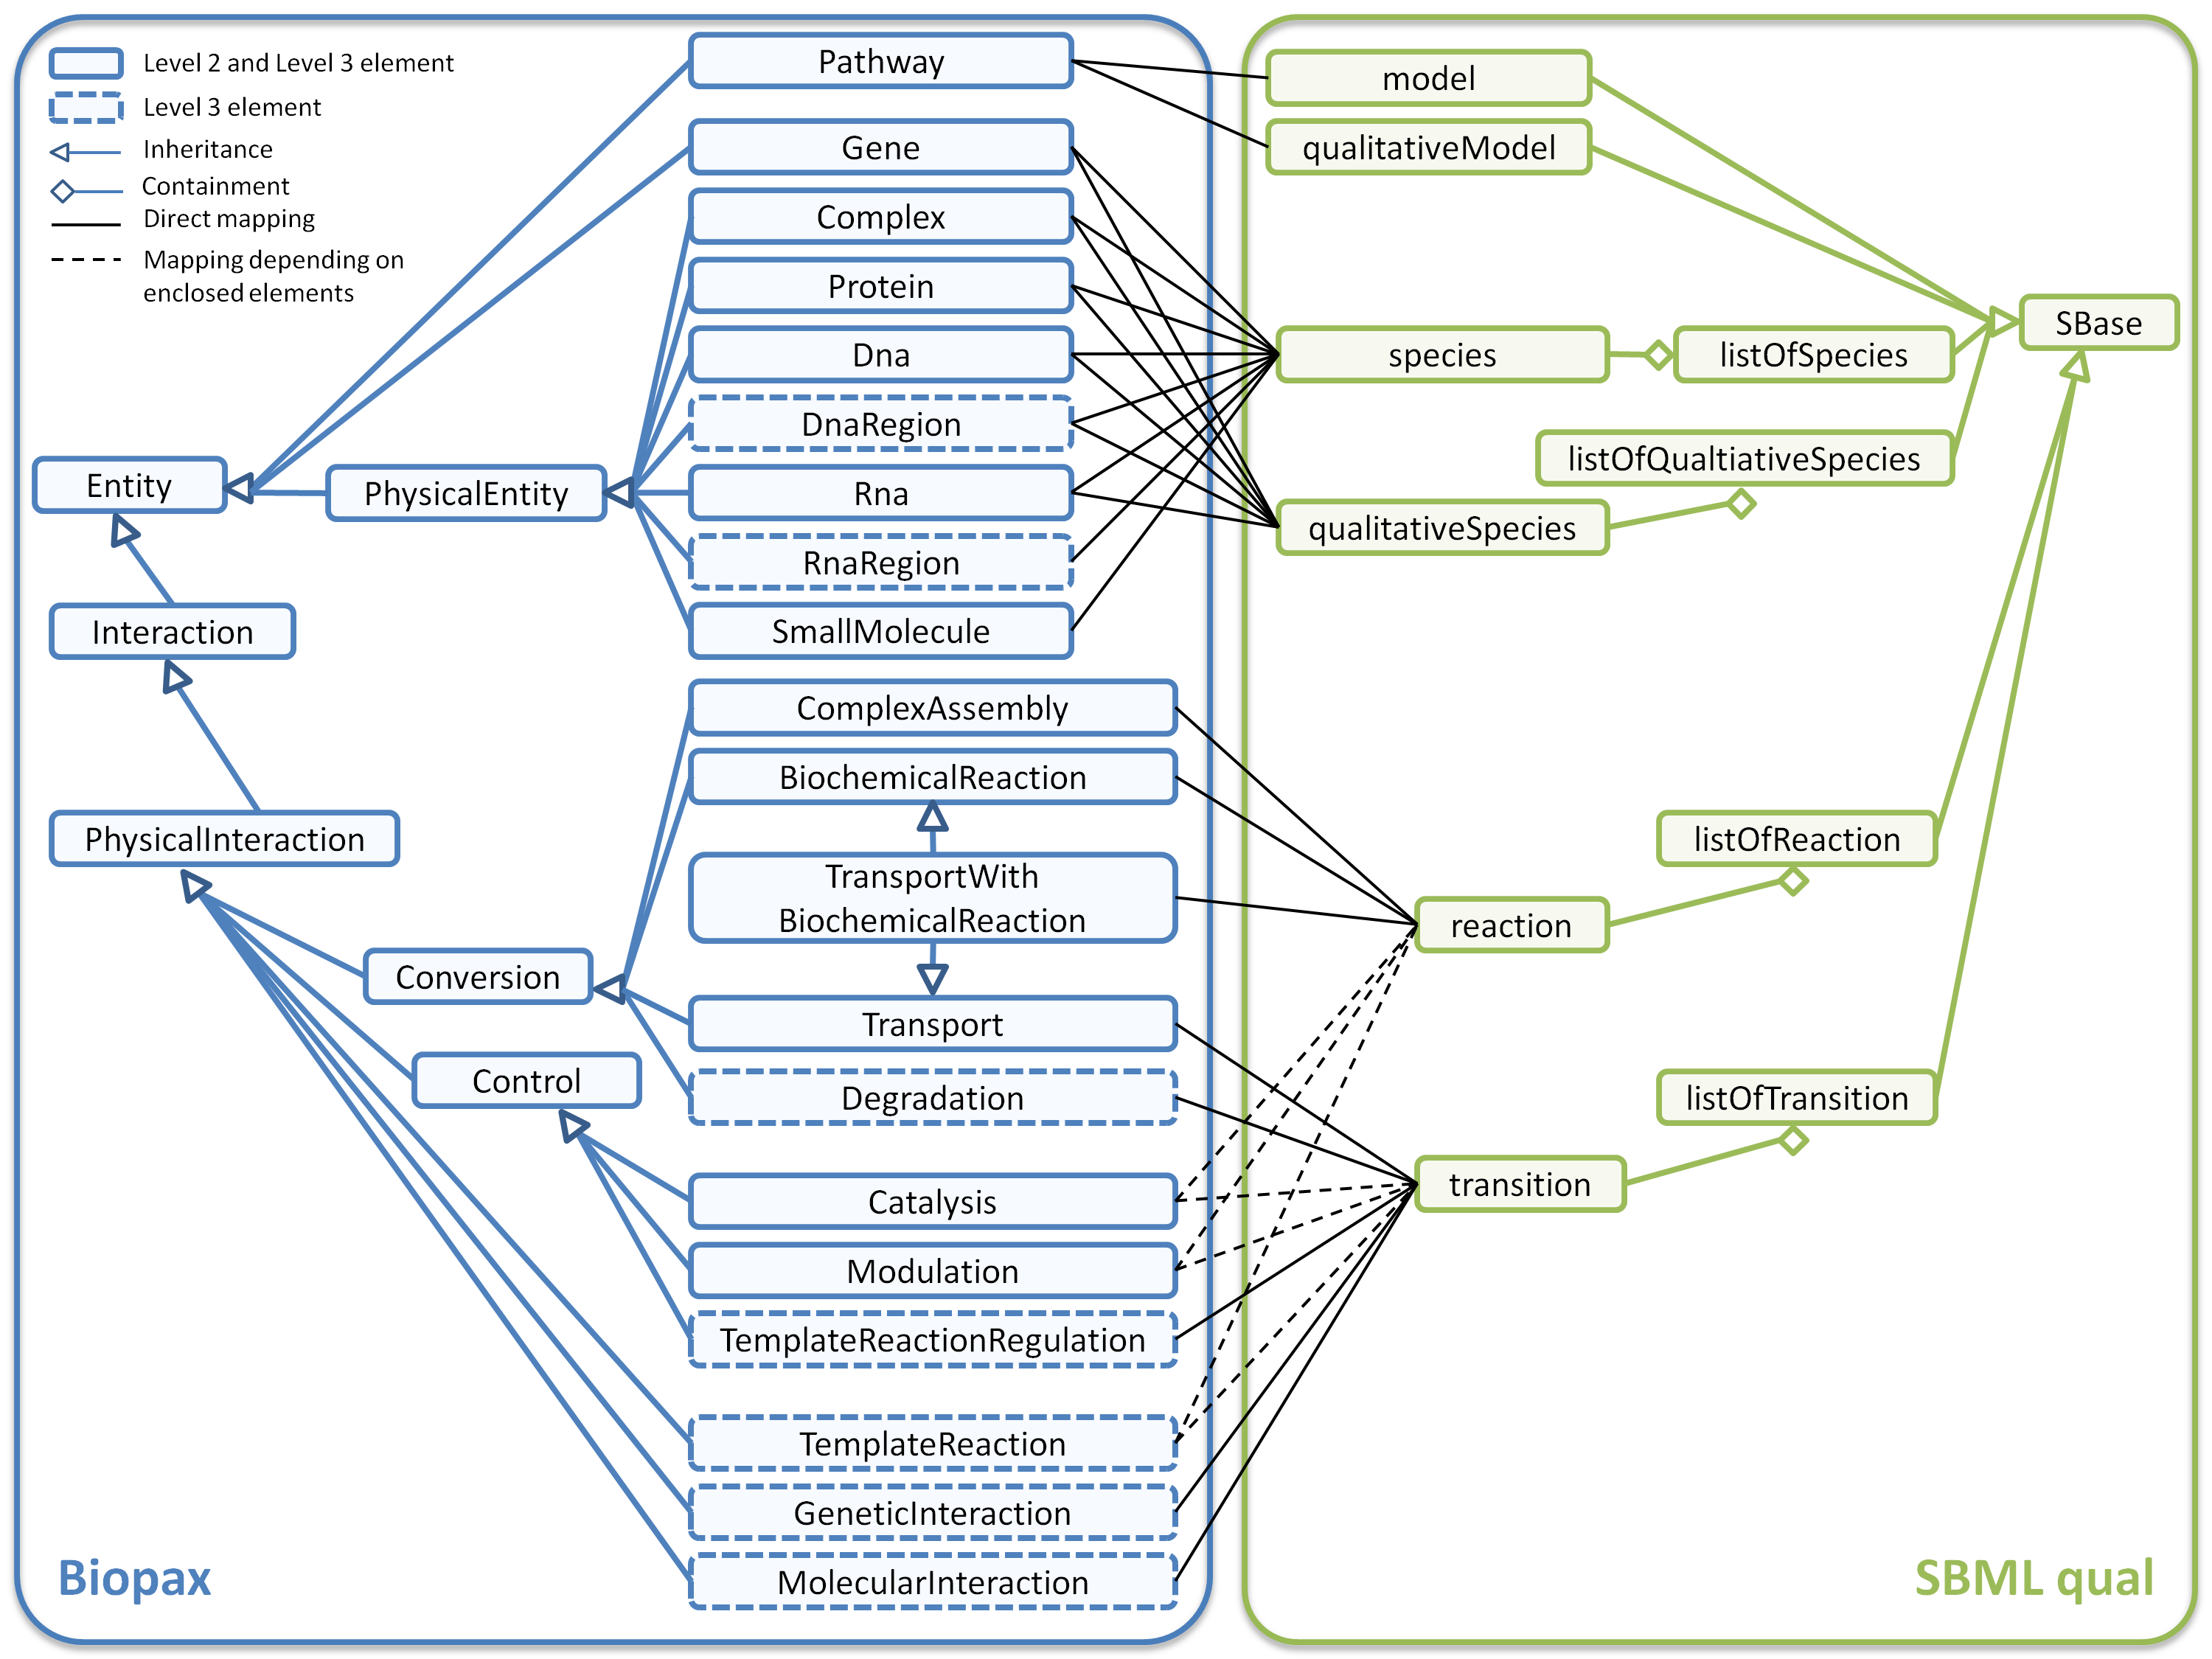
\includegraphics[width=0.95\textwidth]{BioPaxSBMLqual.png}
\caption{Conversion from BioPax Level~2 and Level~3 to SBML with the
Qualitative Models extension (\qual).
The green rounded rectangles describe the SBML and \qual{} classes, and the blue ones the BioPax elements.
The distinction between BioPax Level~2 and Level~3 elements is visualized with dashed rectangles.
The dashed rectangles denote elements, which are only available in Level~3.
All other elements occur in both levels.
%The ancestry of both BioPax and SBML elements is drawn as blue arrows for BioPax respectively with green arrows for SBML.
%If elements are contained in another element this relationship is visualized as a line ending with a diamond.
The ancestry of both BioPax and SBML elements is indicated with arrows.
Lines, ending with a diamond, indicate elements that are contained in other elements.
The conversion from BioPax to SBML \qual{} is drawn with black lines.
For some BioPax elements, it depends on the enclosed entities if the BioPax element is translated into a reaction or to a relation.
This translation dependency is visualized with black dashed lines.
A detailed translation description of those elements is shown in Table~\ref{Tab:BioPax2SBML}.}
\label{fig:BioPaxSBMLqual}
\end{figure*}
%%%%%%%%%%%%%%%%%%%%%%%%%%% END FIGURE 1 %%%%%%%%%%%%%%%%%%%%%%%%%%%%%%%%%%%%%%%%%%%%%%
%%%%%%%%%%%%%%%%%%%%%%%%%%%%%%%%%%%%%%%%%%%%%%%%%%%%%%%%%%%%%%%%%%%%%%%%%%%%%%%%%%%%%%%
The complete nature Pathway Interaction Database (PID) is converted from BioPax to SBML including the Qualitative Models extension.
PID provides curated pahtways from the National Cancer Institute, pathways from BioCarta from June 2004, and human Reactome pathways (Version 22), whereas the Reactome data is updated as soon as new pathway information is available \citep{Schaefer2009}.
The translation of the BioPax Level~2 and Level~3 pathway files is performed in four steps: (1) initialize the model, (2) translation of \PhysicalEntity's, (3) translation of \Interaction's, and (4) annotation of all \species.
An overview of the mapping from BioPax elements to SBML and to SBML \qual{} elements is shown in Figure~\ref{fig:BioPaxSBMLqual}.

%%%%%%%%%%%%%% 1. Step %%%%%% determine organism
\subsubsection{Step 1: Initializing the models}
In the first step, the pathway organism is determined by searching for the BioSource reference in the BioPax file.
%The default organism is human.
Furthermore, the SBML \model{} and \qualitativeModel{} are build.
Both models correspond to the complete pathway represented in the BioPax file.

%%%%%%%%%%%%%% 2. Step %%%%%% entities and annotation
\subsubsection{Step 2: Translation of \PhysicalEntity{} elements}
%%%%%%%%%%%%%%%%%%%%%%%%%%%%%%%%%%%%%%%%%%%%%%%%%%%%%%%%%%%%%%%%%%%%%%%%%%%%%%%%%%%%%%%
%%%%%%%%%%%%%%%%%%%%%%%%%%% TABLE X %%%%%%%%%%%%%%%%%%%%%%%%%%%%%%%%%%%%%%%%%%%%%%%%%
\begin{table}[tb]
\processtable{BioPax \Entity{}'s and assigned SBO terms\label{Tab:BioPax2SBO}}
{\begin{tabular}{llll}\toprule
\textbf{BioPax \Entity} & \textbf{Assigned SBO term} & \textbf{SBO name} \\
\midrule
Gene            & SBO:0000240 & informational molecule segment \\
Complex         & SBO:0000253 & non-covalent complex \\
Protein         & SBO:0000252 & polypeptide chain \\
Dna             & SBO:0000251 & deoxyribonucleic acid \\
DnaRegion       & SBO:0000251 & deoxyribonucleic acid \\
Rna             & SBO:0000250 & ribonucleic acid \\
RnaRegion       & SBO:0000250 & ribonucleic acid \\
SmallMolecule   & SBO:0000247 & simple chemical \\
\botrule
\end{tabular}}
{
Each BioPax \Entity{} is converted to an SBML \species{} and \qualitativeSpecies.
In BioPax, one can specify the nature of the real entity by classes that are derived from \Entity{} (e.g., DNA, Protein, etc).
SBML does not contain specific entities that can be derived from an SBML \species.
The common way to separate different genomic entities in SBML is using SBO terms from the material entity branch.
This table specifies the SBO terms that we used to distinguish between various cellular entities in SBML.
}
\end{table}
%%%%%%%%%%%%%%%%%%%%%%%%%%% END Table 2 %%%%%%%%%%%%%%%%%%%%%%%%%%%%%%%%%%%%%%%%%%%%%%%
%%%%%%%%%%%%%%%%%%%%%%%%%%%%%%%%%%%%%%%%%%%%%%%%%%%%%%%%%%%%%%%%%%%%%%%%%%%%%%%%%%%%%%%

In the second step, an SBML \species{} and \qualitativeSpecies{} is created for each \PhysicalEntity{}.
Depending on the kind of the \PhysicalEntity, i.e., if it is a protein, complex, DNA, RNA, or small molecule, the species is annotated with the corresponding SBO term (\citealp{SBO}, see Table~\ref{Tab:BioPax2SBO} for a list of used terms).

Then, the BioPax document is mined for an RDF link from the \PhysicalEntity{} to a corresponding Entrez Gene ID.
These identifers are unique and facilitate the automated annotation of this species (described in the fourth step).
If there exists no Gene ID but a gene symbol, the gene symbol is mapped to a Gene ID.
%If neither a Gene ID nor a gene symbol is available the name of the \PhysicalEntity{} is used.

%%%%%%%%%%%%%% 3. Step %%%%%% reaction relations
\subsubsection{Step 3: Translation of \Interaction{} elements}
In the third step, the BioPax \Interaction{} elements are converted.
Interaction elements can be split into \Conversion{} and \Control{} elements.

{\Conversion}'s are mainly translated into SBML reactions except the \Transport{} and the \Degradation{} elements, which are translated into transitions.
%%%% Reactions
The translation of reactions from BioPax to SBML is performed by creating the same reaction with all substrates, products and enzymes in SBML.
Furthermore, BioPax Level~3 provides the stoichiometry of the reactants and products of {\BiochemicalReaction}'s and
{\TransportWithBiochemicalReaction}'s, which are also translated into SBML.
Level~2 does not provide stoichiometric information.

%%%%% Control
The translation of the \Conversion{} elements is straightforward, whereas the translation of \Control{} elements is more sophisticated, because translation into a transition or a reaction depends on the enclosed \Control{} elements.
\Control{} elements always consist of zero or more \Controller{} and zero or one \Controlled{} elements.
\Controller{} elements can be inherited from \PhysicalEntity{} or \Pathway, whereas \Controlled{} elements are also \Interaction{} elements.
Thus, it depends on the kind of \Controller{} and the \Controlled{} element whether the \Interaction{} is translated into an SBML reaction or transition.
If the \Controller{} or the \Controlled{} element is a \Pathway{} element, the \Interaction{} is always converted to a transition, because it is biologically not possible to create a reaction with a whole pathway as an reactant or a product.
A \Conversion{} is translated into a \transition{} if the \Controlled{} element is translated into a transition, too.
For instance, the conversion of a \Modulation, consisting of a \PhysicalEntity{} as \Controller{} and a \BiochemicalReaction{} as \Controlled, is translated into a reaction.
An example is shown in Figure~\ref{fig:Ceramide}, which shows the ceramide signaling pathway, where the biochemical reaction from sphingomyelin to ceramide (the \Controlled{} element) is positively modulated from SMPD1+ (the \Controller).
This modulation will be converted into a reaction where SMPD1+ is modeled as an enzyme of the reaction.
But if the \Controlled{} element is a \Degradation, the \Modulation{} is converted into a transition.
In some cases, the \Controlled{} element is an \Interaction{} entity that does not belong to a special subclass.
Then, the \Controlled{} element itself is translated into a transition, and the connection between the \Controller{} and the translated \transition{} is also translated into a transition.
The \sign{} attribute of the \Input{} element describes the relationship between \Input{} and \Output{} and is determined depending on the \ControlType{} attribute.
This attribute is assigned to nearly all \Control{} elements.
If the \ControlType{} is activating, \sign{} is set to \emph{active}; if it is inhibiting \sign{} is set to \emph{negative}; if it is both \sign{} is set to \emph{dual}; otherwise \sign{} is set to \emph{unknown}.
A detailed overview of the conversion of the \Control{} elements is shown in Table~\ref{Tab:BioPax2SBML}.


%%%%%%%%%%%%%%%% Step 4 %%%%% annotation, CLEMENS: MIRIAM und SBO %%%%%%%%%%%%%%
\subsubsection{Step 4: Annotation of the translated model}
%%%%%%%%%%%%%%%%%%%%%%%%%%%%%%%%%%%%%%%%%%%%%%%%%%%%%%%%%%%%%%%%%%%%%%%%%%%%%%%%%%%%%%%%
%%%%%%%%%%%%%%%%%%%%%%%%%%% BEGIN FIGURE 2 %%%%%%%%%%%%%%%%%%%%%%%%%%%%%%%%%%%%%%%%%%%%%
\begin{figure}[t!h]
\centering 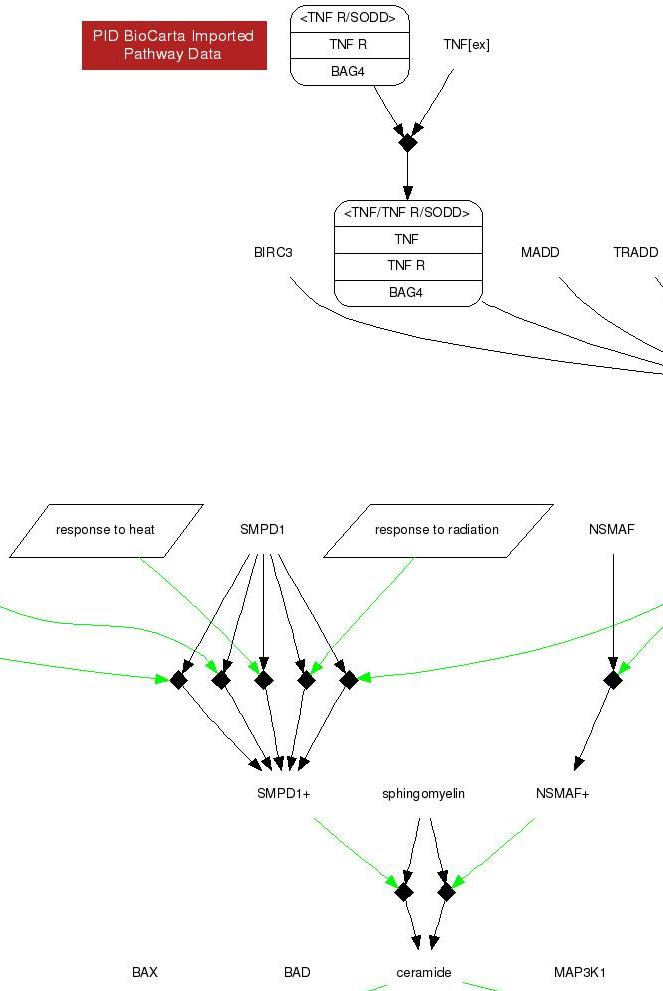
\includegraphics[width=0.85\columnwidth]{CeramidePart.jpg}
\caption{Part of the ceramide signaling pathway imported from BioCarta into the
Pathway Interaction Database (PID).
Modifications are denoted with black diamonds.
The entities with an black arrow to the diamond describe the modulation inputs
and the entities with an black arrow out of the diamond the modulation output.
The green arrows symbolize positive regulators and the round rectangles complexes.
Pathways are visualized with a trapezium.
The ceramide signaling pathway is one pathway example providing an amount of information which cannot be translated to SBML before the recent release of the Qualitative Models extension (\qual).
With \qual, it is possible to translate reactions an relations and to include them in one model.
Even pathway-reaction modulations, like the ``response to heat�� pathway that positively stimulates the reaction from SMPD1 to SMPD1+, can be described.
(Figure by courtesy of the National Cancer Institute -- http://www.cancer.gov).}
\label{fig:Ceramide}
\end{figure}
%%%%%%%%%%%%%%%%%%%%%%%%%%% END FIGURE 2 %%%%%%%%%%%%%%%%%%%%%%%%%%%%%%%%%%%%%%%%%%%%%%%
%%%%%%%%%%%%%%%%%%%%%%%%%%%%%%%%%%%%%%%%%%%%%%%%%%%%%%%%%%%%%%%%%%%%%%%%%%%%%%%%%%%%%%%%
In the fourth and final step, the SBML instances are further annotated.
The BioPax specification allows users to encode arbitrary identifiers for elements.
These can be identifiers for various databases, e.g., UniProt, Entrez Gene, Ensembl, etc.
Unfortunately, the syntax used in BioPax is sometimes inconsistent, which leads to XML database annotations like ``UniProt'' or ``UniProtKB'' within BioPax documents that hamper the automatic reading and interpretation of those models by third party applications.


%%%%%%%%%%% Beispiel %%%%%%%%%%%%%%%%%%%%
%  <bp:unificationXref rdf:ID="unificationXref14">
%    <bp:DB rdf:datatype="http://www.w3.org/2001/XMLSchema\#string">UniProt</bp:DB>
%    <bp:ID rdf:datatype="http://www.w3.org/2001/XMLSchema\#string">Q4KMY3</bp:ID>
%  </bp:unificationXref>
%  <bp:unificationXref rdf:ID="unificationXref14">
%    <bp:DB rdf:datatype="http://www.w3.org/2001/XMLSchema\#string">UniProtKB</bp:DB>
%    <bp:ID rdf:datatype="http://www.w3.org/2001/XMLSchema\#string">Q4KMY3</bp:ID>
%  </bp:unificationXref>
%  <bp:unificationXref rdf:ID="unificationXref14">
%    <bp:DB rdf:datatype="http://www.w3.org/2001/XMLSchema\#string">UniProt</bp:DB>
%    <bp:ID rdf:datatype="http://www.w3.org/2001/XMLSchema\#string">Q4KMY3, Q7Z5L2</bp:ID>
%  </bp:unificationXref>
%%%%%%%%%%% Beispiel ENDE %%%%%%%%%%%%%%%%%%%%

In SBML, such identifiers can be expressed as standardized MIRIAM URNs that can be added as annotation to any SBML element.
We support and add MIRIAM identifiers for the following databases: Entrez Gene, Omim, Ensembl, UniProt, ChEBI, DrugBank, Gene Ontology, HGNC, PubChem, 3DMET, NCBI Taxonomy, PDBeChem, GlycomeDB, LipidBank, EC-Numbers (enzyme nomeclature) and various KEGG databases (gene, glycan, reaction, compound, drug, pathway, orthology).
To obtain identifiers for those databases, we map the Entrez Gene identifier, which we annotated on every element in Step 2, to a KEGG identifier.
Using the KEGG API, we then query all of those identifiers to retrieve more descriptive names, descriptions of the elements, and the mentioned database identifiers.
% CW: Entfernt. wurde durch neuen satz (s.o.) ersetzt.
% All supported identifiers from the BioPax files are parsed, some are manually
% curated by us, and some annotations are supplemented by additional queries to
% the KEGG API for every translated element.
The goal of those annotations is to provide models that can be used directly by
many researchers, no matter what identifiers or databases they use.
\end{methods}


%%%%%%%%%%%%%%%%%%%%%%%%%%%%%%%%%%%%%%%%%%%%%%%%%%%%%%%%%%%%%%%%%%%%%%%%%%%%%%%%%%%%%%%
%%%%%%%%%%%%%%%%%%%%%%%%%%% TABLE 1 %%%%%%%%%%%%%%%%%%%%%%%%%%%%%%%%%%%%%%%%%%%%%%%%%
\begin{table}[t!h]
\processtable{Description of the translation of BioPax \Control{}
elements\label{Tab:BioPax2SBML}} {\begin{tabular}{llll}\toprule
BioPax \Controller & BioPax \Controlled               & Converted\\
                  &                                 & SBML \qual\\
                  &                                 & element\\
\midrule
%\textbf{BioPax Level~3}\\
\multicolumn{3}{c}{\centering \textbf{BioPax Level~3}}\\
\midrule
PhysicalEntity & BiochemicalReaction                & reaction\\
PhysicalEntity & ComplexAssembly                    & reaction\\
PhysicalEntity & Conversion                            & transition\\
PhysicalEntity & Degradation                        & transition\\
PhysicalEntity & Transport                          & transition\\
PhysicalEntity & TransportWithBiochemicalReaction   & reaction\\
PhysicalEntity & Pathway                            & transition\\
PhysicalEntity & TemplateReaction                   & transition\\
\\
Pathway         & BiochemicalReaction               & transition\\
Pathway         & ComplexAssembly                   & transition\\
Pathway         & Conversion                        & transition\\
Pathway         & Degradation                       & transition\\
Pathway         & Pathway                           & transition\\
Pathway         & TemplateReaction                  & transition\\
Pathway         & Transport                         & transition\\
Pathway         & TransportWithBiochemicalReaction  & transition\\
\\\midrule
%\textbf{BioPax Level~2}\\
\multicolumn{3}{c}{\centering \textbf{BioPax Level~2}}\\
\midrule
physicalEntity & biochemicalReaction                & reaction\\
physicalEntity & complexAssembly                    & reaction\\
physicalEntity & interaction                        & transition\\
physicalEntity & pathway                            & transition\\
physicalEntity & transport                          & transition\\
physicalEntity & transportWithBiochemicalReaction   & reaction\\
\\
pathway         & biochemicalReaction               & transition\\
pathway         & complexAssembly                   & transition\\
pathway         & interaction                       & transition\\
pathway         & pathway                           & transition\\
pathway         & transportWithBiochemicalReaction  & transition\\
pathway         & transport                         & transition\\\botrule
\end{tabular}}{BioPax \Control{} elements consists of a \Controller{} and one
or more \Controlled{} elements.
Depending on the kind of \Controller{} or \Controlled{} element, the \Control{} entity is translated into an SBML reaction or transition.
The table gives an overview of this conversion regarding BioPax Level~2 and BioPax Level~3.
The Level~2 entities are labeled with small initial letters and the translation is listed in the lower part of the table.}
\end{table}
%%%%%%%%%%%%%%%%%%%%%%%%%%% END TABLE 1 %%%%%%%%%%%%%%%%%%%%%%%%%%%%%%%%%%%%%%%%%%%%%%%



\subsection{Implementation}
The conversion was programmed with Java\TTra, using JSBML \citep{Draeger2011} with the Qualitative Models extension, PaxTools \citep{Demir2010}, and the KEGG API \citep{Kanehisa2006}.
PaxTools was used to read the BioPax files and to manipulate the information content.
This information was extended with MIRIAM identifiers \citep{Novere2005} for the following databases: Entrez Gene, Omim, Ensembl, UniProt, ChEBI, DrugBank, Gene Ontology, HGNC, PubChem, 3DMET, NCBI Taxonomy, PDBeChem, GlycomeDB, LipidBank, EC-Numbers (enzyme nomeclature) and various KEGG databases (gene, glycan, reaction, compound, drug, pathway, orthology).




\section{Results and Discussion}
% Aufbau:
% Kern problem: BioPax-Format der PID Pathways und die fehlende M�glichkeit
% relationen darzustellen.


% 3. Aber das Format ist ungeeignet
% 4. Daher gibt es mehrere Konverter, die folgendes k�nnen reaction
% 5. Das gen�gt nicht weil wir brauchen relationen
% 6. Jetzt gibt es endlich BioPax to SBML qual, das viel besser ist weil,...
% 7. Im folgenden werden die Merkmale n�her erl�utert.

% 1. PID ist toll weil...
The Pathway Interaction Database (PID) is a curated and peer-reviewed pathway database containing human pathways with molecular signaling and regulatory events provided by the Nature Cancer Institute, BioCarta, and Reactome.
All pathways are provided in XML, BioPax Level~2, and Level~3 format.

% 2. Man k�nnte so viel tun (Simulation, Informationsverkn\"upfung, tolle SBML programme aufz�hlen?, Siehe KGTrans)
% 3. Aber das Format ist ungeeignet
% 4. Daher gibt es mehrere Konverter, die folgendes k�nnen: reaction
The BioPax format is perfectly suitable to encode pathway relations and reactions that can be further used for visualizations or pathway analysis. However, this format also has its limitations. Many applications, especially for simulation and modeling of biological networks, use the SBML format. Therefore, a few importers and converters for BioPax2SBML have been developed. Unfortunately, prior to the release of the SBML Qualitative Models (\qual) extension, it was not possible to properly describe relations in SBML. Hence, the few available converters were either forced to skip the relations, or to create improper pseudo-reactions.

Furthermore, the models themselves just provide the base for further analysis or visualization methods. Other applications focus on visualization, simulation, analysis, etc. of those models. Therefore, most of those applications have certain requirements on the models. For example, to uniquely map mass spectrometry data on a model, it may be required for the model to have UniProt IDs. To match mRNA expression data or perform gene set enrichment analysis, entrez gene identifiers might be required. Consequently, we provide all annotations that we could gather from the input BioPax files also in the SBML files and further annotate all \species{} with a plethora of additional identifiers.


% ALTER TEXT:
%Until now, the pathways are not available in the SBML format and they cannot be translated into SBML without loosing information, because the SBML core specification describes reactions but no other relationships.
%However, the description of those relationships becomes more and more interesting for simulation processes and analysis purposes.
%Many simulation tools use SMBL and not BioPax, although they cannot analyze relations.
%The recently published SBML Qualitative Models extension (\qual) solves this inconvenience and enables the description of such processes in a simple and easily understandable way.

The \qual{} extension has only be recently released and thus, might not be supported by all applications yet. Therefore, we decided to build mixed SBML core and \qual{} models. All our SBML files contain a \model{} that corresponds to the SBML core specification, and an additional \qualitativeModel{} that contains all relations. These models are compatible with older applications, that do not yet support \qual{} but still can read all \species{} and \reaction's. But newer applications that are ready to handle relations can read the additional \qual{} model and process all information that was also available in the BioPax file.


% Whereas other conversion tools cannot translate relations, due to the missing
% SBML specification, we can provide a complete translation of the PID database.
We converted both, the Level~2 and the Level~3 BioPax files to SBML core, including the \qual{} extension. All models are available at \url{http://www.cogsys.cs.uni-tuebingen.de/software/Qualitative-Models/}.
The reason for converting both levels was the additional description possibility of gene regulatory networks and genetic interactions in BioPax Level~3, which is not supported by Level~2 pathway models.

% Kommentiert da info bereits oben erw�hnt wird.
%Since, the models are augmented with additional database information, stored as MIRIAM annotations, the models can easily be used for further simulation purposes. These annotations enable extensive visualization and data exchange between researchers.



\section{Conclusion}
Conversion between different formats is important in all parts of computer sciences.
In many cases converstion leads to errors or a loss of information.
The BioPax to SBML conversion is such an example.
Due to limitations of the SBML specification, it was not possible to include all information from BioPax files in SBML files, while producing
correct SBML code.
But with SBML Level~3 and the addition of extensions to the specifications, in particular the Qualitative Models extension (\qual), it is now possible to create accurate and specification-conform SBML code, and to minimize or even eliminate the loss of information.

BioPax is an RDF format that defines various derived \Entity's which can be genes, proteins, small molecules, etc.
These can be translated into SBML \species{} and the type of the BioPax \Entity{} can be encoded as SBO term or MIRIAM annotation of the species itself.
Relations between \Entity's (which correspond to edges in a pathway picture) are also provided with detailed information in BioPax.
These can be transports, biochemical reactions, complex assemblies, etc.
At this point most transations to SBML usually produce errors or have a massive loss of information.
The SBML core specification only provides reactions, which represents real biochemical reactions with substrates, products and enzymes.
Processes such as the transport or modulation of an entity cannot directly be encoded as a reaction, at least not without knowing the exact chemical equation.
Hence, former conversions approaches from BioPax to SBML did either incorrectly convert those relations to reactions or simply removed them during the translation.
To fill this gap, the SBML community has recently released the \qual{} specification, which allows users to model arbitrary transitions between species.
Using this extension, we produced error-free SBML and minimize or even eliminate the loss of information during the translation.

The SBML models, provided along with this publication, consists of SBML \species and, wherever possible, exact \reaction equations.
Furthermore, all relations from the BioPax documents that could not be converted to exact reactions have been included as qualitative transitions between qualitative species.
Additional information, such as various identifiers or the type of an entity, are encoded as SBO terms or MIRIAM URNs of the corresponding elements.
Furthermore, lots of information is added beyond the scope of the BioPax document by utilizing the KEGG API.

This results in comprehensive and correct SBML models, created for all pathways in the nature pathway interaction database.
The files can be downloaded at \url{http://www.cogsys.cs.uni-tuebingen.de/software/Qualitative-Models/}.
These models can easily be used, e.g., for further simulation and modeling steps, without having to deal with incorrect input file formats or error-prone conversions.

\section*{Acknowledgements}
\paragraph{Funding\textcolon}
Federal Ministry of Education and Research (BMBF, Germany) in the National
Genome Research Network (NGFN+) under grant number 01GS08134 and Virtual Liver
Network unter grant number 0315756.
\paragraph{Conflict of interest\textcolon} None declared.


\bibliographystyle{natbib}
%\bibliographystyle{achemnat}
%\bibliographystyle{plainnat}
%\bibliographystyle{abbrv}
%\bibliographystyle{bioinformatics}
%\bibliographystyle{plain}
%
\begin{thebibliography}{}

\bibitem[Berenguier {\em et~al.}(2011)Berenguier, Chaouiya, Naldi, Thieffry,
  and van Iersel]{QualSpecification}
Berenguier, D., Chaouiya, C., Naldi, A., Thieffry, D., and van Iersel, M.~P.
  (2011).
\newblock {Qualitative Models} (qual).
\newblock Specification available at
  \url{http://sbml.org/Community/Wiki/SBML\_Level\_3\_Proposals/Qualitative\_Models}.
  Accessed 2012 Mar 22.

\bibitem[Courtot {\em et~al.}(2011)Courtot, Juty, Kn\"{u}pfer, Waltemath,
  Zhukova, Dr\"{a}ger, Dumontier, Finney, Golebiewski, Hastings, Hoops,
  Keating, Kell, Kerrien, Lawson, Lister, Lu, Machne, Mendes, Pocock,
  Rodriguez, Villeger, Wilkinson, Wimalaratne, Laibe, Hucka, and
  Nov\`{e}re]{SBO}
Courtot, M., Juty, N., Kn\"{u}pfer, C., Waltemath, D., Zhukova, A., Dr\"{a}ger,
  A., Dumontier, M., Finney, A., Golebiewski, M., Hastings, J., Hoops, S.,
  Keating, S., Kell, D.~B., Kerrien, S., Lawson, J., Lister, A., Lu, J.,
  Machne, R., Mendes, P., Pocock, M., Rodriguez, N., Villeger, A., Wilkinson,
  D.~J., Wimalaratne, S., Laibe, C., Hucka, M., and Nov\`{e}re, N.~L. (2011).
\newblock Controlled vocabularies and semantics in systems biology.
\newblock {\em Mol Syst Biol\/}, {\bf 7}, 543.

\bibitem[Demir {\em et~al.}(2010)Demir, Cary, Paley, Fukuda, Lemer, Vastrik,
  Wu, D'Eustachio, Schaefer, Luciano, Schacherer, Martinez-Flores, Hu,
  Jimenez-Jacinto, Joshi-Tope, Kandasamy, Lopez-Fuentes, Mi, Pichler,
  Rodchenkov, Splendiani, Tkachev, Zucker, Gopinath, Rajasimha, Ramakrishnan,
  Shah, Syed, Anwar, Babur, Blinov, Brauner, Corwin, Donaldson, Gibbons,
  Goldberg, Hornbeck, Luna, Murray-Rust, Neumann, Reubenacker, Samwald, van
  Iersel, Wimalaratne, Allen, Braun, Whirl-Carrillo, Cheung, Dahlquist, Finney,
  Gillespie, Glass, Gong, Haw, Honig, Hubaut, Kane, Krupa, Kutmon, Leonard,
  Marks, Merberg, Petri, Pico, Ravenscroft, Ren, Shah, Sunshine, Tang, Whaley,
  Letovksy, Buetow, Rzhetsky, Schachter, Sobral, Dogrusoz, McWeeney, Aladjem,
  Birney, Collado-Vides, Goto, Hucka, Nov\`{e}re, Maltsev, Pandey, Thomas,
  Wingender, Karp, Sander, and Bader]{Demir2010}
Demir, E., Cary, M.~P., Paley, S. {\em et~al.} (2010).
\newblock The {BioPAX} community standard for pathway data sharing.
\newblock {\em Nat Biotechnol\/}, {\bf 28}(9), 935--942.

\bibitem[Dr\"ager {\em et~al.}(2011)Dr\"ager, Rodriguez, Dumousseau, D\"orr,
  Wrzodek, Le~Nov\`{e}re, Zell, and Hucka]{Draeger2011}
Dr\"ager, A., Rodriguez, N., Dumousseau, M., D\"orr, A., Wrzodek, C.,
  Le~Nov\`{e}re, N., Zell, A., and Hucka, M. (2011).
\newblock {JSBML: a flexible Java library for working with SBML}.
\newblock {\em Bioinformatics\/}, {\bf 27}(15), 2167--2168.

\bibitem[{European Bioinformatics Institute -- Computational Systems
  Neurobiology Group}(2011){European Bioinformatics Institute -- Computational
  Systems Neurobiology Group}]{SBFC}
{European Bioinformatics Institute -- Computational Systems Neurobiology Group}
  (2011).
\newblock {System Biology Format Converter (SBFC)}.
\newblock Software available from
  \url{http://www.ebi.ac.uk/compneur-srv/sbml/converters/SBMLtoBioPax.html}.
  Accessed 2012 Mar 22.

\bibitem[Funahashi {\em et~al.}(2007)Funahashi, Jouraku, Matsuoka, and
  Kitano]{Funahashi2007}
Funahashi, A., Jouraku, A., Matsuoka, Y., and Kitano, H. (2007).
\newblock {Integration of CellDesigner and SABIO-RK.}
\newblock {\em In Silico Biol\/}, {\bf 7}(2 Suppl), S81--S90.

\bibitem[Hucka {\em et~al.}(2003)Hucka, Finney, Sauro, Bolouri, Doyle, Kitano,
  Arkin, Bornstein, Bray, Cornish-Bowden, Cuellar, Dronov, Gilles, Ginkel, Gor,
  Goryanin, Hedley, Hodgman, Hofmeyr, Hunter, Juty, Kasberger, Kremling,
  Kummer, Nov\`{e}re, Loew, Lucio, Mendes, Minch, Mjolsness, Nakayama, Nelson,
  Nielsen, Sakurada, Schaff, Shapiro, Shimizu, Spence, Stelling, Takahashi,
  Tomita, Wagner, Wang, and Forum]{Hucka2003}
Hucka, M., Finney, A., Sauro, H.~M. {\em et~al.} (2003).
\newblock {The systems biology markup language (SBML): a medium for
  representation and exchange of biochemical network models.}
\newblock {\em Bioinformatics\/}, {\bf 19}(4), 524--531.

\bibitem[Kanehisa {\em et~al.}(2006)Kanehisa, Goto, Hattori, Aoki-Kinoshita,
  Itoh, Kawashima, Katayama, Araki, and Hirakawa]{Kanehisa2006}
Kanehisa, M., Goto, S., Hattori, M., Aoki-Kinoshita, K.~F., Itoh, M.,
  Kawashima, S., Katayama, T., Araki, M., and Hirakawa, M. (2006).
\newblock From genomics to chemical genomics: new developments in {KEGG}.
\newblock {\em Nucleic Acids Res\/}, {\bf 34}(Database issue), D354--D357.

\bibitem[Mi {\em et~al.}(2011)Mi, Muruganujan, Demir, Matsuoka, Funahashi,
  Kitano, and Thomas]{Mi2011}
Mi, H., Muruganujan, A., Demir, E., Matsuoka, Y., Funahashi, A., Kitano, H.,
  and Thomas, P.~D. (2011).
\newblock {BioPAX support in CellDesigner.}
\newblock {\em Bioinformatics\/}, {\bf 27}(24), 3437--3438.

\bibitem[Nov\`{e}re {\em et~al.}(2005)Nov\`{e}re, Finney, Hucka, Bhalla,
  Campagne, Collado-Vides, Crampin, Halstead, Klipp, Mendes, Nielsen, Sauro,
  Shapiro, Snoep, Spence, and Wanner]{Novere2005}
Nov\`{e}re, N.~L., Finney, A., Hucka, M., Bhalla, U.~S., Campagne, F.,
  Collado-Vides, J., Crampin, E.~J., Halstead, M., Klipp, E., Mendes, P.,
  Nielsen, P., Sauro, H., Shapiro, B., Snoep, J.~L., Spence, H.~D., and Wanner,
  B.~L. (2005).
\newblock Minimum information requested in the annotation of biochemical models
  {(MIRIAM)}.
\newblock {\em Nat Biotechnol\/}, {\bf 23}(12), 1509--1515.

\bibitem[R\"ubenacker {\em et~al.}(2009)R\"ubenacker, Moraru, Schaff, and
  Blinov]{Ruebenacker2009}
R\"ubenacker, O., Moraru, I.~I., Schaff, J.~C., and Blinov, M.~L. (2009).
\newblock {Integrating BioPAX pathway knowledge with SBML models.}
\newblock {\em IET Syst Biol\/}, {\bf 3}(5), 317--328.

\bibitem[Schaefer {\em et~al.}(2009)Schaefer, Anthony, Krupa, Buchoff, Day,
  Hannay, and Buetow]{Schaefer2009}
Schaefer, C.~F., Anthony, K., Krupa, S., Buchoff, J., Day, M., Hannay, T., and
  Buetow, K.~H. (2009).
\newblock {PID: the Pathway Interaction Database.}
\newblock {\em Nucleic Acids Res\/}, {\bf 37}(Database issue), D674--D679.

\bibitem[Smoot {\em et~al.}(2011)Smoot, Ono, Ruscheinski, Wang, and
  Ideker]{Smoot2011a}
Smoot, M.~E., Ono, K., Ruscheinski, J., Wang, P.-L., and Ideker, T. (2011).
\newblock Cytoscape 2.8: new features for data integration and network
  visualization.
\newblock {\em Bioinformatics\/}, {\bf 27}(3), 431--432.

\bibitem[Zinovyev {\em et~al.}(2008)Zinovyev, Viara, Calzone, and
  Barillot]{Zinovyev2008}
Zinovyev, A., Viara, E., Calzone, L., and Barillot, E. (2008).
\newblock {BiNoM: a Cytoscape plugin for manipulating and analyzing biological
  networks.}
\newblock {\em Bioinformatics\/}, {\bf 24}(6), 876--877.

\end{thebibliography}


\end{document}
